%!TeX root=../tese.tex
%("dica" para o editor de texto: este arquivo é parte de um documento maior)
% para saber mais: https://tex.stackexchange.com/q/78101

%!TeX root=../tese.tex
%("dica" para o editor de texto: este arquivo é parte de um documento maior)
% para saber mais: https://tex.stackexchange.com/q/78101

\chapter{Conexidade em grafos dinâmicos}

\enlargethispage{.8\baselineskip}

\section{Definição}

Como citado no Capítulo~1, o problema da conexidade em grafos dinâmicos visa construir um algoritmo eficiente que dá suporte a inserções, remoções e consultas de conexidade. O algoritmo de Holm, de Lichtenberg e Thorup~\cite{jacob_holm} para este problema de conexidade é composto por $\left\lceil \lg n \right\rceil$ florestas dinâmicas do grafo $G$, e utiliza uma biblioteca que será descrita na Subseção 2.2. 

\section{Conexidade em florestas dinâmicas}

Rodrigues \cite{arthur}, em sua dissertação do mestrado, estudou, entre outros assuntos, o problema da conexidade em florestas dinâmicas e implementou o seu algoritmo, que foi proposto na Seção~2 do artigo de Holm, de Lichtenberg e Thorup~\cite{jacob_holm}. No Capítulo~2 da sua dissertação ele descreve as rotinas principais do algoritmo, baseado em \textit{Euler tour trees}, e realiza uma análise minuciosa da complexidade de tempo das funções dos pseudocódigos. Dada essas circunstâncias, optamos por não apresentar uma descrição detalhada desse algoritmo, explicando brevemente sobre o que as rotinas principais fazem, bem como algumas diferenças da nossa implementação em código comparadas com a de Rodrigues.  

O problema da conexidade em florestas dinâmicas pode ser considerada uma simplificação do problema de conexidade em grafos dinâmicos, quando o grafo em questão é uma floresta. A biblioteca que usaremos contém os seguintes métodos:

\begin{itemize}
    \item \texttt{\textbf{florestaDinâmica(F, n)}}: constrói e devolve uma floresta dinâmica $F$ com $n$ vértices isolados;
    \item \texttt{\textbf{conectadosFD(F, u, v)}}: devolve verdadeiro se \textit{u} e \textit{v} estão na mesma componente da floresta $F$ e falso caso contrário;
    \item \texttt{\textbf{adicioneFD(F, u, v)}}: insere uma aresta \textit{uv} na floresta $F$;
    \item \texttt{\textbf{removaFD(u, v)}}: remove a aresta \textit{uv} da floresta $F$;
\end{itemize}

A estrutura de dados principal usada neste algoritmo de Holm, de Lichtenberg e Thorup~para dar suporte eficientes às rotinas acima é uma árvore binária de busca balanceada (ABBB). Dessa forma, a floresta dinâmica é constituída de várias ABBBs. Rodrigues utiliza \textit{treaps} em sua implementação, que é de natureza aleatória. Em nosso caso, utilizamos árvores \textit{splay}, que foram desenvolvidas por \textit{Sleator e Tarjan} \cite{sleator}. Árvores \textit{splay} são árvores binárias de busca (ABBs) que possuem uma rotina extra (além das usuais de busca, inserção e remoção) chamada \textit{splay}, que é acionada ao final de cada operação feita na árvore, de modo que é sempre aplicada ao nó mais profundo visitado. Isso faz com que o custo amortizado da operação \textit{splay} seja $O(\lg n)$, onde $n$ é o número de nós da árvore, e que também uma sequência de $m$ acessos em uma árvore \textit{splay} tenha custo total $O(m \lg n)$.  Como também já existe bastante literatura sobre árvores \textit{splay}, e seu funcionamento interno não afeta a descrição dos algoritmos que descreveremos, não entraremos em detalhes de sua implementação.

\section{Estrutura da implementação do grafo dinâmico}

Para implementar o grafo dinâmico, resume-se à construção da seguinte biblioteca de forma eficiente:

\begin{itemize}
    \item \texttt{\textbf{grafoDinâmico(G, n)}}: contrói e devolve um grafo dinâmico $G$ com $n$ vértices isolados;
    \item \texttt{\textbf{conectadosGD(G, u, v)}}: devolve verdadeiro se os vértices $u$ e $v$ estão na mesma componente de $G$ e falso caso contrário;
    \item \texttt{\textbf{adicioneGD(G, u, v)}}: adiciona a aresta $uv$ no grafo $G$;
    \item \texttt{\textbf{removaGD(G, u, v)}}: remove a aresta $uv$ do grafo $G$.
\end{itemize} 

Nossa implementação encapsula a complexidade de manutenção de $\left\lceil \lg n \right\rceil$ florestas dinâmicas em uma abstração do grafo dinâmico. 
Assim, a consulta \texttt{conectadoGD} aplicada ao grafo $G$ significa fazer a mesma consulta para alguma floresta maximal $F$ de $G$. Dessa maneira, sempre que estivermos realizando alguma operação de alteração ou consulta de conexidade em nosso grafo $G$, estamos também a realizando em uma floresta dinâmica $F$ que seja maximal em $G$. Da mesma forma, quando chamamos o construtor do grafo dinâmico, estamos criando $\left\lceil \lg n \right\rceil$ florestas de vértices isolados.

\section{Adição de arestas no grafo dinâmico}

Quando realizamos uma chamada à função \texttt{adicioneGD}, é feita uma chamada ao \texttt{conectadoGD} para verificar a conexidade de $u$ com $v$ em $G$. Se estes vértices não estiverem ligados em $G$, então é inserido a aresta $uv$ na floresta maximal que estamos mantendo, assim ligando a árvore que contém $u$ com a que contém $v$ nessa floresta. Chamamos essas arestas de \textbf{arestas da floresta}.

Caso $u$ e $v$ já estiverem conectados em $G$, então essa aresta $uv$ é chamada de \textbf{aresta reserva} e ela será armazenada em um grafo representado por listas de adjacências, que contém a seguinte biblioteca:

\begin{itemize}
    \item \texttt{\textbf{listaDeAdjacências(L, n)}}: constrói e devolve um grafo $L$ contendo $n$ listas de adjacências, onde $n$ é o número de vértices isolados;
    \item \texttt{\textbf{adicioneLA(L, u, v)}}: adiciona $u$ na lista de adjacências de v em $L$ e vice-versa;
    \item \texttt{\textbf{removaLA(L, u, v)}}: remove $u$ da lista de adjacências de $v$ em $L$ e vice-versa.
\end{itemize} 

A nossa implementação \cite{chung2025} para lista de adjancências possui um custo O($n$) ao acionar o construtor \texttt{listaDeAdjacências}, e para 
as rotinas \texttt{adicioneLA} e \texttt{removaLA} são garantidos o tempo esperado O($1$) visto que estamos utilizando um mapa hash da linguagem \textit{C++} para realizar adição de um vizinho $v$ em $u$ e, se houver, remoção de $v$ da lista de adjancência de $u$.

Como a inserção de arestas (\texttt{adicioneFA}) em uma floresta dinâmica com $n$ vértices possui uma complexidade de tempo esperado O(lg$n$), então temos que \texttt{adicioneGD} também terá o seu custo esperado de tempo O(lg$n$). 

O objetivo de guardar arestas reservas em nosso grafo é simples. Seja o grafo $G$ com $V = \{a, b, c, d, e, f, g\}$ e suas respectivas arestas, como ilustrado na Figura~\ref{fig:graph_without_reserve_edges}. Temos dois subgrafos $G_1$ e $G_2$ em nosso grafo $G$. O vértice $a$ está em $G_1$ e $e$ está em $G_2$. Se $G_1$ e $G_2$ são conectados por uma única aresta $ae$, a remoção dela acarretaria em duas componentes separadas. Então chamar \texttt{conectado(G, a, e)} após a remoção de $ae$ receberíamos falso como resposta. 

\begin{figure}
    \centering
    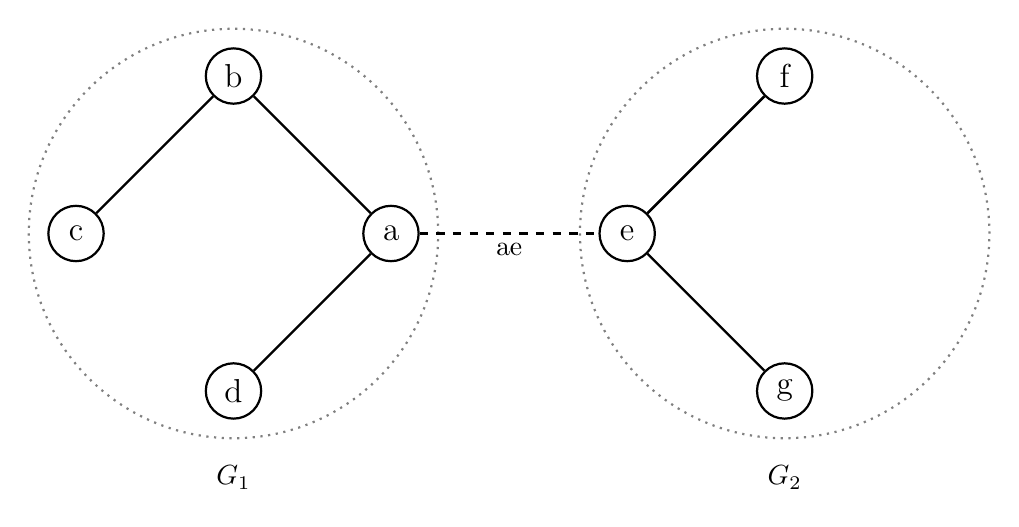
\begin{tikzpicture}
        [node/.style={circle,draw,minimum size=2em, thick, font=\large},
        edge/.style={thick, black},
        reserve/.style={red, very thick, dashed},
        removed/.style={black, thick, dashed}]

        % Vertices in a circular arrangement
        \node[node] (a) at (-1,2) {a};
        \node[node] (b) at (-3,4) {b};
        \node[node] (c) at (-5,2) {c};
        \node[node] (d) at (-3,0) {d};
        \node[node] (e) at (2,2) {e};
        \node[node] (f) at (4,4) {f};
        \node[node] (g) at (4,0) {g};
        
         % Dotted circles for T_u and T_v
        \draw[dotted, thick, gray] (-3,2) circle (2.6cm); % T_u circle around {a,b,c,d}
        \draw[dotted, thick, gray] (4,2) circle (2.6cm);  % T_v circle around {e,f,g}
        
        % Labels for the circles
        \node at (-3,-1.1) {$G_1$};
        \node at (4,-1.1) {$G_2$};


        % tree edges (normal black edges)
        \draw[edge] (a) -- (b) node[midway, below] {};
        \draw[edge] (b) -- (c) node[midway, below] {};
        \draw[edge] (a) -- (d) node[midway, below] {};
        \draw[edge] (e) -- (f) node[midway, below] {};
        \draw[edge] (e) -- (f) node[midway, below] {};
        \draw[edge] (e) -- (g) node[midway, below] {};
        \draw[removed] (a) -- (e) node[midway, below] {ae};

        % MST edges ( in red)
        %\draw[reserve] (d) -- (g) node[midway, below] {dg};
        
    \end{tikzpicture}
    \caption{Um grafo com sete vértices e sem nenhuma aresta reserva. O subgrafo $G_1$ contém os vértices $a$, $b$, $c$ e $d$, enquanto $G_2$ contém os vértices $e$, $f$ e $g$. A aresta tracejada $ae$ está prestes a ser removida.}
    \label{fig:graph_without_reserve_edges}
\end{figure}

Agora, suponha que $G_1$ e $G_2$ eram componentes conexas separadas, e foram  conectadas pela aresta $ae$, tornando-se uma única componente conexa, como mostra a Figura~\ref{fig:graph_with_reserve_edges}. Ao chamarmos \texttt{adiciona(G, d, g)}, guardaríamos a aresta $dg$ como reserva. Se posteriormente removermos $ae$, note que os subgrafos $G_1$ e $G_2$ estariam em duas componentes separadas. Assim, se não tivéssemos armazenado $dg$, então a consulta \texttt{conectado(G, a, e)} devolveria falso, o que estaria incorreto visto que a aresta $dg$ existe de fato no grafo. Dessa forma, a aresta reserva possui a função de substituir a aresta removida, como veremos adiante, mantendo a conexão entre $G_1$ e $G_2$.

\begin{figure}
    \centering
    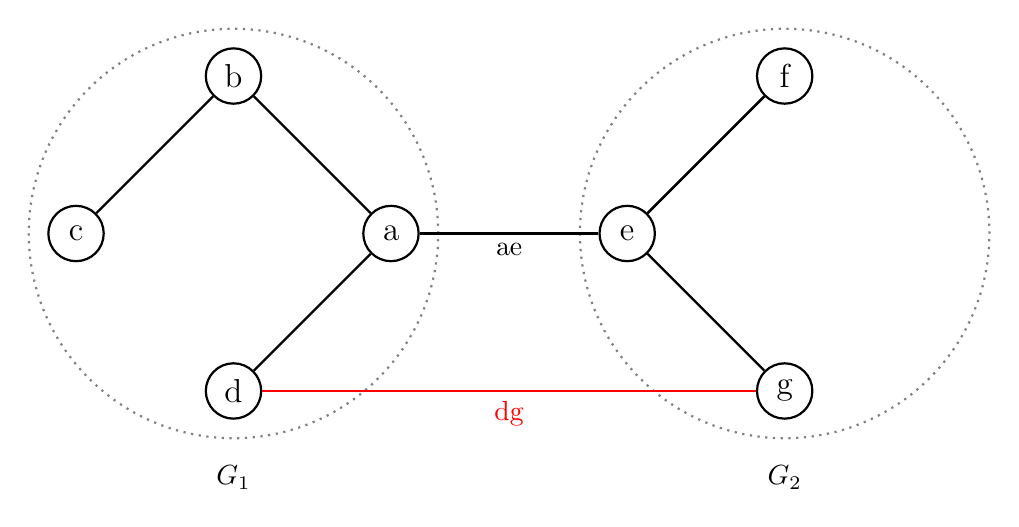
\begin{tikzpicture}
        [node/.style={circle,draw,minimum size=2em, thick, font=\large},
        edge/.style={thick, black},
        reserve/.style={red, thick},
        removed/.style={black, thick, dashed}]

        % Vertices in a circular arrangement
        \node[node] (a) at (-1,2) {a};
        \node[node] (b) at (-3,4) {b};
        \node[node] (c) at (-5,2) {c};
        \node[node] (d) at (-3,0) {d};
        \node[node] (e) at (2,2) {e};
        \node[node] (f) at (4,4) {f};
        \node[node] (g) at (4,0) {g};
        
         % Dotted circles for T_u and T_v
        \draw[dotted, thick, gray] (-3,2) circle (2.6cm); % T_u circle around {a,b,c,d}
        \draw[dotted, thick, gray] (4,2) circle (2.6cm);  % T_v circle around {e,f,g}
        
        % Labels for the circles
        \node at (-3,-1.1) {$G_1$};
        \node at (4,-1.1) {$G_2$};


        % tree edges (normal black edges)
        \draw[edge] (a) -- (b) node[midway, below] {};
        \draw[edge] (b) -- (c) node[midway, below] {};
        \draw[edge] (a) -- (d) node[midway, below] {};
        \draw[edge] (e) -- (f) node[midway, below] {};
        \draw[edge] (e) -- (f) node[midway, below] {};
        \draw[edge] (e) -- (g) node[midway, below] {};
        \draw[edge] (a) -- (e) node[midway, below] {ae};

        % MST edges ( in red)
        \draw[reserve] (d) -- (g) node[midway, below] {dg};
        
    \end{tikzpicture}
    \caption{Um grafo com sete vértices. O subgrafo $G_1$ contém os vértices $a$, $b$, $c$ e $d$, enquanto $G_2$ contém os vértices $e$, $f$ e $g$. A aresta vermelha $dg$ é uma aresta reserva do grafo.}
    \label{fig:graph_with_reserve_edges}
\end{figure}

Note que não podemos simplesmente adicionar $dg$ como aresta da floresta maximal de $G$ em vez de guardar nas listas de adjacências. Como por definição uma floresta não pode conter ciclos, adicionar $dg$ dada a existência da aresta $ae$ acarretaria na formação de um ciclo contendo essas duas arestas, o que violaria a estrutura do algoritmo, já que queremos manter árvores binárias de busca balanceadas para garantir a complexidade de tempo logarítmica em suas rotinas. Como um grafo pode conter ciclos, guardar a aresta como reserva é uma forma de manter o grafo correto e o algoritmo eficiente. 

\section{Remoção de arestas no grafo dinâmico}

Dessa forma, quando queremos remover uma aresta reserva, podemos simplesmente acionar a rotina \texttt{removaLA} (da lista de adjacências) e a floresta maximal do grafo não será afetada. Entretanto, se queremos remover uma aresta $uv$ do grafo $G$, a floresta é quebrada em duas componentes, que podemos chamar de árvores $T_u$ e $T_v$, de modo que o primeiro contém o vértice $u$ e o segundo contém o vértice $v$. Dessa forma, precisamos verificar se existe alguma aresta reserva que liga $T_u$ a $T_v$, para que possamos garantir que o teste de conexidade de $u$ e $v$ esteja correto. Assim, precisamos procurar uma aresta reserva que irá substituir a aresta que foi removida de $G$, que vamos chamar de \textbf{aresta substituta}.

Podemos supor, sem perda de generalidade, que $|T_u| \leq |T_v|$, ou seja, o número de vértices de $T_u$ é no máximo o de $T_v$. Assim, para procurar uma aresta reserva que substitua a removida, precisaríamos percorrer cada vértice $x$ de $T_u$ e verificar se existe algum vértice $y$ na lista de adjacências de $x$, de modo que $y$ esteja em $T_v$. Se $y \in V(T_v)$, teríamos encontrado uma aresta substituta $xy$, bastando apenas acionar \texttt{adicioneGD(G, x, y)} para conectar os dois vértices e, consequentemente, $T_u$ e $T_v$ virariam uma única componente da floresta.

\begin{figure}
    \centering
    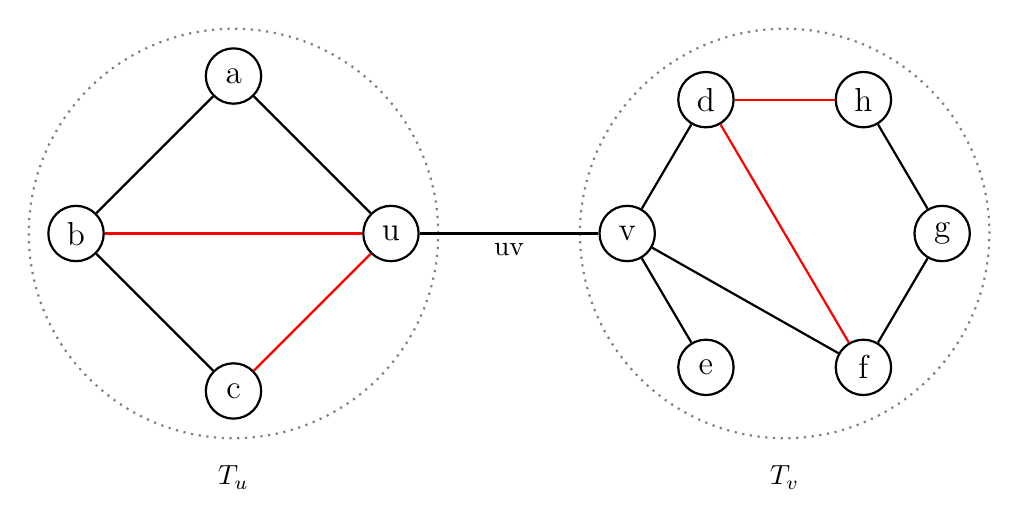
\begin{tikzpicture}
        [node/.style={circle,draw,minimum size=2em, thick, font=\large},
        edge/.style={thick, black},
        reserve/.style={red, thick},
        removed/.style={black, thick, dashed}]

        \node[node] (u) at (-1,2) {u};
        \node[node] (a) at (-3,4) {a};
        \node[node] (b) at (-5,2) {b};
        \node[node] (c) at (-3,0) {c};
        \node[node] (v) at (2,2) {v};
        \node[node] (d) at (3,3.7) {d};
        \node[node] (e) at (3,0.3) {e};
        \node[node] (f) at (5,0.3) {f};
        \node[node] (g) at (6, 2) {g};
        \node[node] (h) at (5, 3.7) {h};
        
        
         % Dotted circles for T_u and T_v
        \draw[dotted, thick, gray] (-3,2) circle (2.6cm);
        \draw[dotted, thick, gray] (4,2) circle (2.6cm);  
        
        % Labels for the circles
        \node at (-3,-1.1) {$T_u$};
        \node at (4,-1.1) {$T_v$};

        % tree edges (normal black edges)
        \draw[edge] (a) -- (u) node[midway, below] {};
        \draw[edge] (a) -- (b) node[midway, below] {};
        \draw[edge] (b) -- (c) node[midway, below] {};
        \draw[edge] (v) -- (d) node[midway, below] {};
        \draw[edge] (v) -- (f) node[midway, below] {};
        \draw[edge] (v) -- (e) node[midway, below] {};
        \draw[edge] (u) -- (v) node[midway, below] {uv};
        \draw[edge] (f) -- (g) node[midway, below] {};
        \draw[edge] (g) -- (h) node[midway, below] {};

        % reserve edges (normal red edges)
        \draw[reserve] (b) -- (u) node[midway, below] {};
        \draw[reserve] (c) -- (u) node[midway, below] {};
        \draw[reserve] (d) -- (f) node[midway, below] {};
        \draw[reserve] (d) -- (h) node[midway, below] {};

    \end{tikzpicture}
    \caption{Um grafo com 10 vértices. As arestas pretas são da floresta maximal do grafo, enquanto as vermelhas são arestas reservas.}
    \label{fig:graph_with_Tu_and_Tv}
\end{figure}

\newpage

Após a remoção da aresta $uv$, note que teremos duas componentes do grado $G$ separadas em $T_u$ e $T_v$. Na Figura~\ref{fig:graph_with_Tu_and_Tv}, por exemplo, não temos uma aresta reserva que ligue $T_u$ e $T_v$. Sob essas condições, suponha que temos um vértice $w \in V(T_u)$ e $z \in V(T_v)$. Assim, ao chamarmos \texttt{conectadoGD(G, w, z)}, note que precisaremos percorrer cada vértice $a$ de $T_u$, e para cada vizinho $b$ de $a$ teríamos que verificar se $b \in V(T_v)$. Assim, o consumo de tempo esperado para essa busca exaustiva é de O($n^2$), visto que supusemos que não há nenhuma aresta reserva que ligue $T_u$ e $T_v$. Como \texttt{conectadoGD} tem consumo de tempo esperado O(lg$n$), então teremos um consumo de O($n^2$lg$n$) para \texttt{removaGD}, pois precisamos verificar se as duas pontas de cada aresta reserva estão conectadas chamando a rotina \texttt{conectadoGD}. Note que achamos uma aresta substituta caso as duas pontas da aresta reserva não estejam conectadas, pois uma delas estará em $T_u$ e outra estará em $T_v$.

Assim, torna-se necessário uma implementação mais eficiente para a rotina de remoção de arestas, e por isso apresentaremos a solução de Holm, de Lichtenberg e Thorup~\cite{jacob_holm}, que resolve este problema em O(lg$^2n$).

\begin{figure}
    \centering
    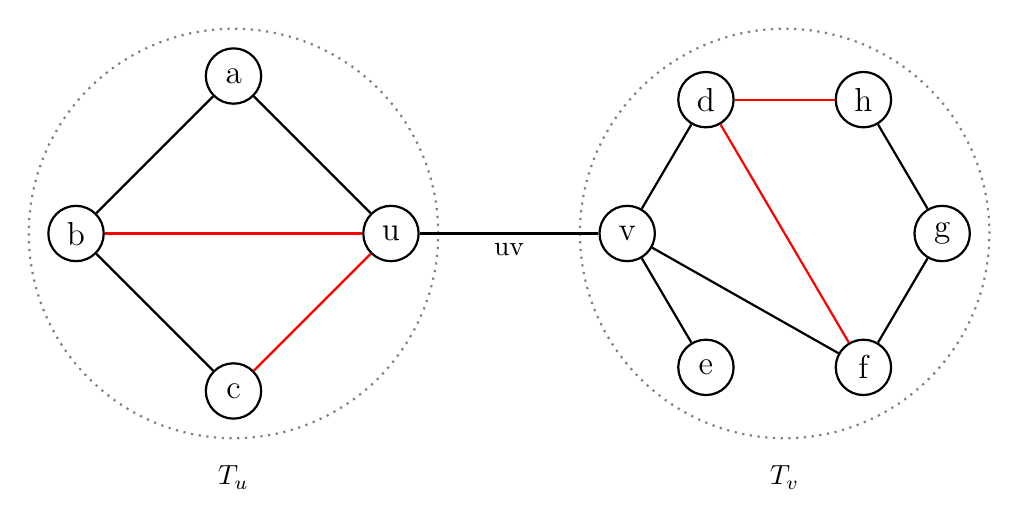
\begin{tikzpicture}
        [node/.style={circle,draw,minimum size=2em, thick, font=\large},
        edge/.style={thick, black},
        reserve/.style={red, thick},
        removed/.style={black, thick, dashed}]

        \node[node] (u) at (-1,2) {u};
        \node[node] (a) at (-3,4) {a};
        \node[node] (b) at (-5,2) {b};
        \node[node] (c) at (-3,0) {c};
        \node[node] (v) at (2,2) {v};
        \node[node] (d) at (3,3.7) {d};
        \node[node] (e) at (3,0.3) {e};
        \node[node] (f) at (5,0.3) {f};
        \node[node] (g) at (6, 2) {g};
        \node[node] (h) at (5, 3.7) {h};
        
        
         % Dotted circles for T_u and T_v
        \draw[dotted, thick, gray] (-3,2) circle (2.6cm);
        \draw[dotted, thick, gray] (4,2) circle (2.6cm);  
        
        % Labels for the circles
        \node at (-3,-1.1) {$T_u$};
        \node at (4,-1.1) {$T_v$};

        % tree edges (normal black edges)
        \draw[edge] (a) -- (u) node[midway, below] {};
        \draw[edge] (a) -- (b) node[midway, below] {};
        \draw[edge] (b) -- (c) node[midway, below] {};
        \draw[edge] (v) -- (d) node[midway, below] {};
        \draw[edge] (v) -- (f) node[midway, below] {};
        \draw[edge] (v) -- (e) node[midway, below] {};
        \draw[edge] (u) -- (v) node[midway, below] {uv};
        \draw[edge] (f) -- (g) node[midway, below] {};
        \draw[edge] (g) -- (h) node[midway, below] {};

        % reserve edges (normal red edges)
        \draw[reserve] (b) -- (u) node[midway, below] {};
        \draw[reserve] (c) -- (u) node[midway, below] {};
        \draw[reserve] (d) -- (f) node[midway, below] {};
        \draw[reserve] (d) -- (h) node[midway, below] {};

    \end{tikzpicture}
    \caption{Um grafo com 10 vértices. As arestas pretas são da floresta maximal do grafo, enquanto as vermelhas são arestas reservas.}
    \label{fig:graph_with_Tu_and_Tv_with_reserve_edge}
\end{figure}

\newpage

\section{Fatiamento do grafo em níveis}

Cada aresta do grafo possui um nível entre $0$ e $\left\lceil \lg n \right\rceil$, onde $n$ é o número de vértices do grafo $G$. Toda vez que inserimos uma aresta em $G$, ela possuirá o nível $\left\lceil \lg n \right\rceil$, e ele nunca será aumentado. Assim, o nível da aresta somente será decrementado quando estamos buscando uma aresta substituta. 

Dessa forma, podemos definir um grafo $G_i$, que é gerador das arestas de nível $\leq i$. Além disso, podemos definir uma floresta maximal de $G_i$.
